\documentclass[12pt]{article}
\usepackage{fullpage,graphicx,psfrag,amsmath,amsfonts,verbatim}
\usepackage[small,bf]{caption}

\input defs.tex

\bibliographystyle{alpha}

\title{\LaTeX\ Style Guide for EE 364B}
\author{Stephen Boyd \and Ernest K. Ryu \and Neal Parikh}

\begin{document}
\maketitle

\begin{abstract}
This document lays out rules and guidelines for mathematical writing and
typesetting that you must follow for your project proposals, reports,
and the final exam, all of which \emph{must} be typeset in \LaTeX. The guidelines
here cover both the \LaTeX\ source as well as the output, so this PDF is
intended to be read alongside its own source code.

There are many well-known references on mathematical writing, but the
goal here is to briefly survey this topic and to lay out some rules specific to
this course. Parts of this document were inspired by or lifted from Halmos
\cite{Halmos:1970} and Knuth \cite{Knuth:1989}.
\end{abstract}

\newpage
\tableofcontents
\newpage

While you are writing, it is often useful to include 
the table of contents so you can see the structure of your document,
even if you don't include it in the final version.

\section{Style guidelines}

You will likely find that attempting to write things out will reveal that you
were not as clear about your topic as you thought you were. John von
Neumann once said, ``There's no sense in being precise when you don't even know
what you're talking about,'' and Niels Bohr wrote, ``Never express yourself more
clearly than you can think.'' Keep these in mind.

Many respectable books follow similar rules, like
\cite{BoV:04},
\cite[p.~23]{Cover:1991},
\cite[p.~26]{Hastie:2001},
\cite[p.~21]{Sipser:2001},
\cite[p.~25]{Cormen:2001},
\cite[p.~15]{Rudin:1976},
\cite[p.~18]{Evans:2010},
\cite[p.~3]{Goldstein:1980}, and 
\cite{Knuth:1973}.

\paragraph{Write good English.}
Always write good English, ``even'' when the subject is mathematics. This
includes correct grammar, word choice, punctuation, spelling, phrasing,
and common sense. 
A classic on this topic, only slightly dated, 
is Strunk and White \cite{SW:59}.

\paragraph{Keep the reader in mind.} Perhaps the most important principle of
good writing is to keep the reader in mind: What do they know so far? What do
they expect next and why? Do they have sufficient motivation for stated
results? As part of this, make sure you know what level of reader you are
writing for and stay consistent with that level. If the reader is expected to
know convex analysis, do not keep defining standard concepts like subgradients.

\paragraph{Write to allow skipping over formulas.}
Many readers will first read through the paper ignoring or skipping all but the
simplest formulas. Your sentences and overall paper should flow smoothly, and
make sense, when all but the simplest formulas are replaced by ``blah'' or a
similar placeholder.  As a related point, do not simply display a list of
formulas or equations in a row; tie the concepts together with a running
commentary.

\paragraph{Be precise with your language.}
The sentence ``Let $x^\star$ be the solution to the optimization
problem'' implicitly asserts that the solution is unique. If the solution is
not unique or need not be unique, write, ``Let $x^\star$ be a solution to the
optimization problem.'' Similarly, do not refer to ``solving'' an expression,
as this is meaningless.  You can solve an equation or set of equations,
evaluate an expression or function, or check that an equation or inequality
holds.

\paragraph{Use the editorial we when appropriate.}
The word ``we'' is often useful to avoid passive voice, which can
sometimes be awkward, or the use of ``I'' or
``one'', which should be avoided. However, be careful not to overuse
``we'', as it can become a very bad habit.
\begin{quote}
Often bad: We can see that Theorem 1 implies Corollary 2.\\
Good: Theorem 1 implies Corollary 2.
\end{quote}
In general, use whatever phrasing makes the sentence cleaner and less clunky.
To quote Strunk and White, ``Omit needless words.''

\paragraph{Punctuation in equations.}
An equation is part of a sentence, and you may need to include a comma or a period
at the end of an equation as a result, whether or not you are using inline or
display math style. For example:
\begin{quote}
    We next discuss how to solve the problem
    \[
        \begin{array}{ll}
            \mbox{minimize} & (1/2)\|Ax - b\|_2^2,
        \end{array}
    \]
    where $x \in \reals^n$ is the optimization variable.
\end{quote}

\paragraph{Don't start a sentence with a symbol.}
This hurts readability:
\begin{quote}
Bad: $f$ is smooth.\\
Good: The function $f$ is smooth.

Bad: $x^n - a$ has $n$ distinct zeros. \\
Good: The polynomial $x^n - a$ has $n$ distinct zeros.
\end{quote}
Similarly, don't start a sentence with a reference.

\paragraph{Use words to separate symbols in different formulas.}
If it might confuse the reader visually or in the actual
meaning of the sentence, use words to break apart formulas:
\begin{quote}
Bad: The sequences $x_1, x_2, \dots$, $y_1, y_2, \dots$ are Cauchy. \\
OK: The sequences $x_1, x_2, \dots,$ and $y_1, y_2, \dots,$ are Cauchy. \\
Good: The sequences $(x_i)$ and $(y_i)$ are Cauchy.

OK: The image of $S$ under $f$, $f(S) = \{ x \mid x \in S \}$, is convex. \\
Good: The image of $S$ under $f$, given by $f(S) = \{ x \mid x \in S \}$, is convex.
\end{quote}
Do not insert superfluous words if the meaning is clear.
\begin{quote}
Good: Consider the function $f + g + h$, where $f : \reals^n \to
\reals$, $g : \reals^m \to \reals$, and $h : \reals^p \to \symm^n$ are closed
proper convex.
\end{quote}

\paragraph{References.}
For internal references, use the \texttt{label} and \texttt{ref} commands.
\emph{Never} number or refer to an entity using a specific number,
as in ``Table~3.''
Refer to ``Table~\ref{t-ex1}'', ``\eqref{e-opt-prob}'' (an equation), and so on.
Only number equations that are important and should be emphasized or that you
specifically refer to elsewhere. Do not simply number all equations, and do not
number them randomly. A numbered equation draws the reader's attention, so it
should be used relatively sparingly. Use \verb+\S+ for section references, as in
\S\ref{s-content}.

For external references, you must use Bib\TeX. Use references like nouns or 
footnotes:
\begin{quote}
Good: One useful reference is \cite{BoV:04}. \\
Good: Interested readers may refer to Boyd and Vandenberghe \cite{BoV:04}.
\end{quote}

Your Bib\TeX\ source must be correct.  Unfortunately, many systems that export
Bib\TeX\ entries export very poor ones.  Bib\TeX\ ignores the \texttt{*.bib}
file's capitalization for articles (but not books). To force capitalization,
you must wrap the letter with curly braces.  The hyphen (-), en dash (--), and
em dash (---) are distinct punctuation marks that serve different purposes.
(And the minus sign is different from all three.) When specifying a page range
in references, use the en dash. For an example of escaping and using the en
dash, look at our Bib\TeX\ entry for \cite{Tref:2008}.

\paragraph{Do not italicize English in math mode.}
Mathematical symbols should be typeset in math mode:
write $Ax=b$, not Ax=b. This said, subscripts or
superscripts that derive from English (or any human language) should not be
italicized. For example, write $f_\mathrm{best}$, not $f_{best}$. The exception
is subscripts based on a single letter: refer
to a point that is the center of some set as $x_c$, not $x_{\mathrm{c}}$.
Similarly, use commands for special functions: use $\sin(x)$,
$\log(x)$, and $\exp(x)$, not $sin(x)$, $log(x)$, or $exp(x)$.

A really heinous example would be the following:
\begin{quote}
Consider the problem
\[
\begin{array}{ll}
minimize & f(Ax - b) \\
\end{array}
\]
where x is the optimization variable and A and b are problem data.
\end{quote}

\paragraph{Spacing.}
A blank line ends a paragraph. You shouldn't leave a blank line between an
equation and the following text unless you intend the equation to end the
paragraph. Write:
\begin{quote}
\begin{verbatim}
The image of $S$ under $f$,
\[
    f(S) = \{ f(x) \mid x \in S \},
\]
is convex.
\end{verbatim}
\end{quote}
Inserting extra blank lines before \verb+\[+ or after \verb+\]+ will result in
bad typesetting. However, the following is fine, since a new paragraph is called for:
\begin{quote}
\begin{verbatim}
The image of $S$ under $f$ is defined as
\[
    f(S) = \{ f(x) \mid x \in S \}.
\]

We now turn to a different topic.
\end{verbatim}
\end{quote}
Using a tab before \verb+f(S)+ inside the equation environment is
optional, but helps readability in the source.  Similar rules should be
followed for other environments like \texttt{quote}; see the source of this
document.

\paragraph{Use of notation and jargon.}
The correct and appropriate use of notation and jargon takes time to master.
The following should give you a sense of what to think about:

\begin{itemize}
\item Don't use the same notation for two different things. Conversely, be consistent
about notation for the same thing mentioned in two places: don't
say ``$A_j$ for $1 \leq j \leq n$'' in one place and ``$A_i$ for $i=1,\ldots,n$'' 
in another, or use two different indices in summations over the same ranges. 
Formally, the $i$ and $j$ are dummy variables with only that phrase as scope,
so these are technically correct, but it will confuse the reader.

\item It can be useful to choose names for indices so, for example, $i$
always varies from 1 to $m$ and $j$ always varies from 1 to $n$ (when
referencing something like the rows and columns of an $m \times n$ matrix).

\item Define all symbols before or near to where you use them.  A good rule is that
when you first use something, say, $X$, you should either define it immediately, or 
within the paragraph.   There are a few cases where it is acceptable to define it 
later, but you must say this explicitly, as in ``$X$ is the matrix of activation
levels, which we define below.''

\item A symbol like $f$ refers to a function, while $f(x)$ refers to a
function evaluated at a given point. Avoid sloppy writing like ``The function
$f(x)$ is convex.''
So-called `anonymous' functions defined inline are an exception to this rule,
as in ``the function $x^2 \cos x$ is a counterexample,'' though this should
be used only for simple functions.

\item Use typographic naming conventions like capital letters for sets, Greek
letters for dual variables, \emph{etc}.

\item Try to use mnemonic notation, so $x_c$ for a center point,
$c$ for a cost vector, $S$ for a generic set, $C$ for a convex set, $B$
for a ball, and so on. Note that there are conventions about
the use of different letters in mathematics that you should not ignore:
$i$, $j$, and $k$ are usually used for indices, $x$ through $z$ for
variables, $a$ through $d$ for constants, \emph{etc}.

\item Don't use symbols like $\forall$, $\exists$, and $\Rightarrow$; use the
corresponding words. These symbols are usually appropriate only in
formal logic. 

\item Don't overuse subscripts. If you do not need to assign a subscript
to something, don't. For example, if you begin by defining a set as
$X = \{x_1, \dots, x_n\}$, then it is going to get annoying to refer to subsets
of $X$, since you will need double subscripts. If possible, it would be better
to not name the elements of $X$ and only refer to them when necessary, just
as, say, $x$ and $y$. 

Beware especially of any topic in graph theory when it comes to this rule;
there are often \emph{many} ways to refer to relevant objects, and finding
reasonable notation can often get one half the way to getting a handle on the
problem itself.

\item Don't assign symbols to concepts that you never refer to, or can easily
refer to without:
\begin{quote}
Bad: Let $X$ be a compact subset of a space $Y$. If $f$ is a continuous
real-valued function over $X$, it has a minimum over $X$. \\
Good: A continuous real-valued function has a minimum over a compact set.
\end{quote}
Similarly, do not say ``The solution $x^\star$ is unique'' if you never need
to refer to $x^\star$ again; simply say that the solution is unique.
When you say ``The solution $x^\star$ is unique'' you are both stating a fact
\emph{and} entering the symbol $x^\star$ into the paper's symbol table and
the reader's working memory.
\end{itemize}

\paragraph{Sections.}
Use structures like \texttt{section}, \texttt{subsection},
\texttt{subsubsection}, and \texttt{paragraph} to organize the exposition;
never insert manual line breaks or page breaks for this purpose. In particular,
do not use line breaks to separate different topics. Do not use symbols in
article titles and ideally not even in section headers.

\paragraph{Use capitalization consistently.}
For section headers, capitalize the first letter, proper nouns, and lowercase
everything else, as in this document.  For references, write Figure 1, Algorithm 3,
Theorem 4, and so on.

\paragraph{Use the right commands.}
There are certain special commands in \LaTeX\ for notation that you otherwise
might attempt to write in an ad-hoc manner. If you do the latter, the typesetting
will be inferior. A few common examples:
\begin{itemize}
\item Norms are written $\|x\|$, not $||x||$. 

\item For set-builder notation, use
$\{ x \in \reals \mid x \geq 0 \}$, not $\{x \in \reals | x \geq 0 \}$.

\item Make sure to use \verb+\left+ and \verb+\right+ when wrapping
taller expressions with parentheses, curly braces, brackets, and so on.
\begin{quote}
Bad: Let
\[
    x = \argmin_u (f(u) + \frac{1}{2}\|u - z\|_2^2).
\]
Good: Let
\[
    x = \argmin_u \left(f(u) + \frac{1}{2}\|u - z\|_2^2\right).
\]
\end{quote}

\item Use \verb+\ldots+ (lower dots) when the dots are surrounded by commas and
\verb+\cdots+ (center dots) when surrounded by other objects that have full
height, as in $x_1, x_2, \ldots, x_n$ and $x_1 + x_2 + \cdots + x_n$.
\end{itemize}
Similarly, make sure to use our conventions for standard mathematical objects
for this class; for example, use $\reals$, not $\mathbb{R}$, to denote the set
of real numbers. Use the \verb+\argmin+ and \verb+\argmax+ commands (as shown
above); do not write `arg min', since `argmin' is a single mathematical
operator.  These and other definitions are provided in \verb+defs.tex+.

\paragraph{Writing optimization problems.}
In this class, optimization problems can be introduced in the sentence as
nouns. For example, write as follows:
\begin{quote}
Consider the problem
    \begin{equation}
    \begin{array}{ll}
    \mbox{minimize}   & (1/2)\|Ax-b\|_2^2 + \lambda \|x\|_1 \\
    \mbox{subject to} & 0 \preceq x \preceq \ones \\
    & \|x\|_2 \leq 1,
    \end{array}
    \label{e-opt-prob}
    \end{equation}
where $x \in \reals^n$ is the optimization variable, and $A \in \reals^{m
\times n}$, $b \in \reals^m$, and $\lambda > 0$ are problem data.
\end{quote}
It is important to state which symbols refer to variables and which to problem data.

Be sure to carefully distinguish an optimization problem, 
an algorithm for solving it, and its optimal value.
You \emph{solve} a problem (possibly, using a particular algorithm);
an optimization problem \emph{has} an optimal value;
and an optimization problem \emph{is} convex, or infeasible.
It does not make sense to talk about whether or not a problem converges.

\paragraph{Sentence-ending periods.}
\LaTeX\ assumes all periods followed by a space are sentence-ending periods.
Tell it otherwise when that is not the case.
\begin{quote}
Bad: Let $x_1,x_2,\ldots ,x_n$ be  i.i.d. normal random variables.\\
Good: Let $x_1,x_2,\ldots ,x_n$ be  i.i.d.\ normal random variables.
\end{quote}

\paragraph{Commas.}
Know when commas should appear inside or outside math environments:
\begin{quote}
Bad: Note that $a,b,$ and $c$ are nonnegative.\\
Good: Note that $a$, $b$, and $c$ are nonnegative.

Bad: We conclude that $x_1$, $x_2$, \dots, $x_n$ are decreasing.\\
Good: We conclude that $x_1, x_2, \ldots, x_n$ is decreasing.\\
Good: We conclude that $x_1>x_2> \cdots >x_n$.
\end{quote}

\paragraph{Tables and figures.}
Generally, do not refer to figures or tables in a
way that depend on their placement on the page; give them a \texttt{label}
and then use \texttt{ref} to refer to it. All figures and tables should have
captions.
\begin{quote}
Bad: Properties of several functions are shown in the table below.\\
Good: Properties of several functions are shown in Table~\ref{t-ex1}.
\end{quote}

\begin{table}
\begin{minipage}{\textwidth}
\centering
\begin{tabular}{|c|c|c|}
\hline
$f(x)$      & convex? & differentiable? \\ \hline
$\|x\|_2^2$ & Y       & Y \\
$\|x\|_1$   & Y       & N \\
$\|x\|_2^3$ & N       & Y \\
\hline
\end{tabular}
\caption{Example table}
\label{t-ex1}
\end{minipage} 
\end{table}

\paragraph{\LaTeX\ in figures.}
Generally, mathematical symbols embedded in figures should be rendered by
\LaTeX. In Python, matplotlib has native support for \LaTeX\ rendering.
Otherwise, you can export the image in eps format and use the \LaTeX\ package
psfrag. See Figure~\ref{f-nopsfrag} and Figure~\ref{f-psfrag}. To use psfrag,
compile using
\begin{quote}
\begin{verbatim}
$ latex template.tex
$ dvipdf template.dvi
\end{verbatim}
\end{quote}
The psfrag package does not work with pdflatex.

\begin{figure}
\begin{center}
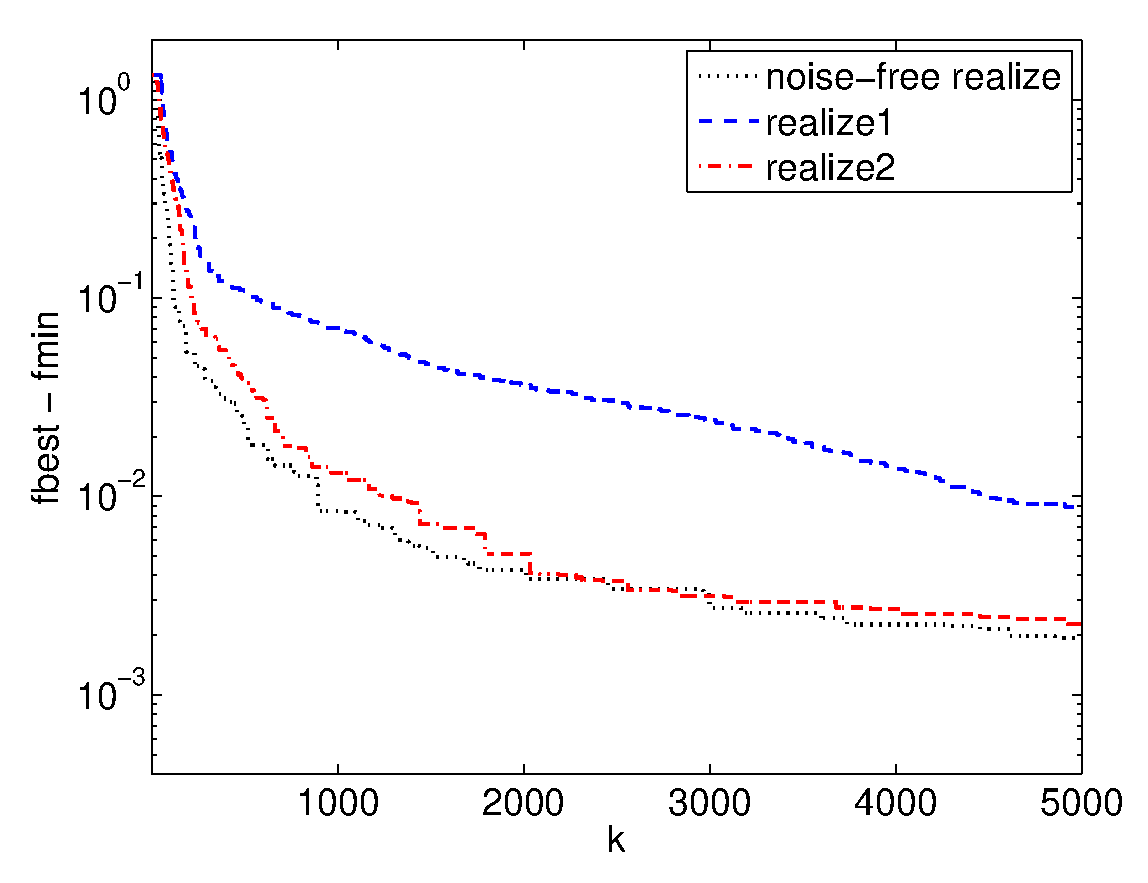
\includegraphics[width=0.6\textwidth]{figures/pwl_error_fbest_realize}
\end{center}
\caption{Original image without psfrag.}
\label{f-nopsfrag}
\end{figure}

\begin{figure}
\begin{center}
\psfrag{k}[t][b]{$k$}
\psfrag{fbest - fmin}[b][t]{$f_\mathrm{best}^{(k)} - f^\star$}
\psfrag{noise-free realize}{noise-free case}
\psfrag{realize1}{realization 1}
\psfrag{realize2}{realization 2}
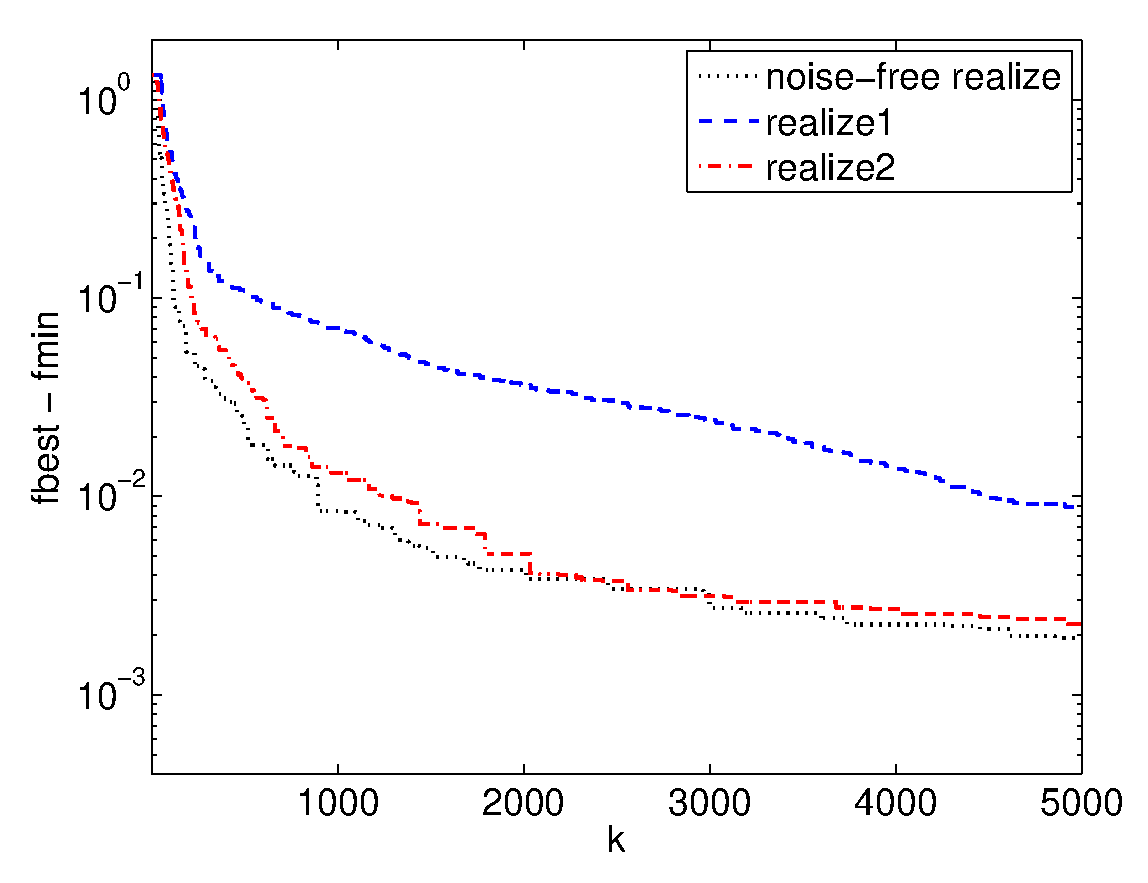
\includegraphics[width=0.6\textwidth]{figures/pwl_error_fbest_realize}
\end{center}
\caption{Text replaced with equations using psfrag.}
\label{f-psfrag}
\end{figure}

\paragraph{Dialects.}
Be aware when you are writing in a mathematical dialect, like statistics,
machine learning, signal processing, control, finance, vision, information
theory, and so on.  Unless your intended audience is only from this one field,
try to avoid using dialect; try to write in such a way that a general reader
with a good understanding of basic mathematics can understand what you are
saying.  If you use terms like CVAR, hinge loss, Bode plot, or IIR filter,
you're speaking dialect. It's very easy to define these things so a person with
knowledge of basic mathematics can understand. Similarly, use standard variable
notation unless otherwise needed: $x$ for variables, $A$ for matrices, and so
on. Don't write a whole paper about solving a linear system you call $\Xi \beta =
\chi$ unless you really need to.

\paragraph{No rule is absolute.}
Break any of these rules rather than write anything nasty.

\section{Source code}

In this example, we show how to include code in a document.
\verbatiminput{example.m}
Here, we could now include some discussion about the code, include plots it
generates, and so on. Use your judgment about whether to start a new page
before displaying code, as it is helpful to be able to display all the code on
a single page. For very short snippets of code (just a few lines), it can help
readability to wrap it in a \texttt{quote} environment.

\section{Content} 
\label{s-content}

Your report should use the following structure:

\begin{enumerate}
\item Begin with a brief paragraph that provides background, perhaps in
somewhat field-specific language.  Describe the problem you hope to address
in general terms.  For example:  ``We consider the problem of
reconstructing an image, given a blurred noisy version of it.'' Ideally,
this opening should be snappy and interesting, otherwise you will lose the
intended audience.

\item Transition (quickly) into a mathematical problem statement that
anyone with general mathematical training can look at and understand,
without any domain knowledge.

\item Outline the general approach. As a general comment here, it is of the
\emph{utmost importance} not to mix together the problem statement and the
method you intend to use to solve instances of that problem. You should cover
these in separate paragraphs, if not separate sections or subsections. This is
a key conceptual point, not just about writing.

Note that the approach is not merely the optimization algorithm you will
eventually use. For example, your approach to solving a nonconvex problem may
be to produce a particular convex relaxation whose solution will give a
heuristic solution for the original problem. Here, the relaxation is as much a
part of the approach as the algorithm you use to solve the relaxation.

\item If relevant, discuss properties of your overall approach, such
as convergence, rate of convergence, implementation details, and so on.
This could be as simple as saying that you use CVX,
or something more involved for, say, a distributed ADMM implementation.
Make sure you explain what machine and software you used.

\item If relevant, present some numerical experiments. If the focus is on an
algorithm, it is important to
thoroughly describe the problem data and settings of any algorithm parameters
(step sizes, stopping criteria, and so on). You should include number of
iterations to convergence, wall-clock time to convergence, residuals at
convergence, and any other related metrics. If appropriate, compare your method
to some relevant baseline, like CVX.
If the focus is on solving a practical problem, describe the 
problem instance (or instances) solved, where the data came from, and so on.
The general problem statement should have been stated before, so when you present
the numerical example, you should not need to define a new problem.
For example:
\begin{quote}
We now consider a specific instance of the index tracking problem~(13).  We
have $n=100$ assets, with daily return data from January 2005 to January 2012,
all obtained from Google Finance.  The transaction cost parameter $\kappa$ was
set to $0.002$, \emph{i.e.}, 20 basis points, which is consistent with typical
transaction costs in practice.
\end{quote}

Typically you would describe the actual \emph{results} in a different paragraph.

\item If your original problem is in a particular field, make sure to try to
pause at various points in the exposition to provide interpretations of the
mathematical properties, approach, or numerical results back in the original
domain.

\item Briefly conclude and summarize the high-level points.
\end{enumerate}

\section*{Acknowledgments}

This is an example of an unnumbered section.

\newpage
\bibliography{template}

\end{document}
